\section{Dropout}
Overfitting'i azaltmak için kullanılan bir düzenleme tekniğidir. Ağın öğrenme sürecinde rastgele seçilen nöronları devre dışı bırakarak ağın genelleme yeteneğini artırır. Bu, ağın farklı altkümelerini kullanarak birden fazla model öğrenmesini simüle eder. Bu süreç boyunca, her bir nöronun çıktısına "dropout" olasığı uygulanır. Bu olasılık nöronun eğitim sırasında geçerli iterasyonda kullanılmama olasılığını belirler. Genelde tam bağlı katmanlardan sonra kullanılarak bağlar koparılır. Böylece düğümler birbirleri hakkında daha az bilgiye sahip olur, birbirleri arasındaki ağırlık değişimlerinden daha az etkilenirler. Dropout, modelin tek bir nörona veya küçük bir nöron grubuna aşırı bağımlı olmasını engeller ve modelin daha geniş bir şekilde öğrenmesini sağlar. Eğitim sırasında nöronlar rastgele devre dışı bırakılır, ancak bu işlem test sırasında yapılmaz. Eğitim sırasında her bir nöronun kapatılma olasılığı $p$, aktif kalma olasılığı $1 - p$'dir. Test sırasında ağırlıklar $(1 - p)$'ye göre ölçeklendirilir.

\begin{figure}[h]
    \centering
    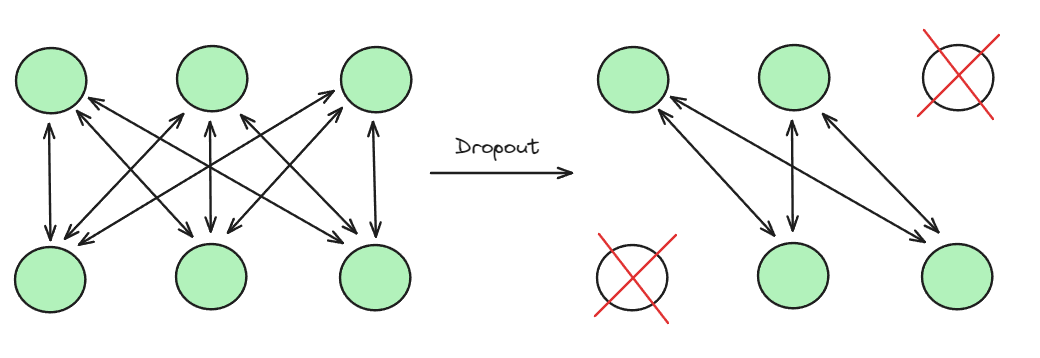
\includegraphics[width=0.6\textwidth]{images/dropout_layer.png}
    \caption{Dropout katmanı.}
    \label{fig:enter-label}
\end{figure}

\subsection{Spatial Dropout}

Spatial Dropout'un klasik Dropout'tan farkı, tüm filtreyi aynı anda devre dışı bırakmasıdır, yani konvolüsyon katmanlarında bir nöron yerine tüm kanalı devre dışı bırakır. Konvolüsyonel katmanlarda, her kanal  tek bir varlık olarak kabul edilir. Spatial Dropout bu kanallardan bazılarını rastgele devre dışı bırakır. Eğitim sırasında, belirli bir oranla tüm bir filtre veya kanal sıfırlanır ve bu kanalın etkisi o geçişte tamamen sıfırlanmış olur. Spatial Dropout, pikselleri yerel ilişkileriyle birlikte (yani tüm kanalı) devre dışı bıraktığı için konvolüsyonel katmanların uzaysal bilgilerini korur ve daha etkili bir regularization yöntemi sunar.

\subsection{Gaussian Dropout}

Normal Dropout, belirli bir nöronun tamamen sıfırlanmasına neden olurken, Gaussian Dropout her bir nöronun çıkışına bir gauss dağılımından (normal dağılım) gelen küçük rastgele bir gürültü ekler. Gaussian Dropout'ta, her bir nöronun çıkışına rastgele bir normal dağılım ile örneklenen bir değer eklenir. Normal Dropout'un aksine, Gaussian Dropout her nöronu tamamen kapatmaz, bunun yerine nöronun etkisini azaltan veya artıran küçük bir varyasyon uygular.

\subsection{Alpha Dropout}

Alpha Dropout, Self-Normalizing Neural Networks (SNN) gibi modellerde kullanılan bir dropout türüdür. SELU (Scaled Exponential Linear Units) aktivasyon fonksiyonlarıyla birlikte çalışmak üzere tasarlanmıştır. SELU aktivasyon fonksiyonları, ağın kendi kendine normalleşmesini sağlar, yani her katmandan gelen aktivasyonlar belirli bir ortalama ve varyansa sahip olur. Bu, modelin her katmandaki sinyali normalize etmesini ve eğitim sırasında istikrarı artırmasını sağlar. Alpha Dropout, Dropout uygularken SELU'nun bu normalleştirici etkisini bozmaz. Kapattığı nöronların aktivasyon değerlerini uygun şekilde ölçeklendirir ve modelin normalizasyon sürecini korur.

\newpage